\documentclass{article}
\usepackage[utf8]{inputenc}

\title{Homework 6}
\author{Compsci 571}
\date{Due Date: April 2018}

\usepackage{natbib}
\usepackage{graphicx}
\usepackage{amsmath}
\usepackage{booktabs}
\usepackage{amsfonts}
\graphicspath{{figures/}}
\usepackage{caption}
\usepackage{subcaption}

\begin{document}

\maketitle

\section{Neural Networks and Universal Approximation Theorem}
\subsection{}
Universal Approximation Theorem states that a single-layer neural network (NN) can be used to approximate any continuous function within certain precision. For any function with one input $x$ and one output $f(x)$, one way to approximate it is to construct several "bumps" as shown in Fig.~\ref{fig:approximation_1d}.

\begin{figure}[h!]
\centering
\begin{subfigure}{.54\textwidth}
  \centering
  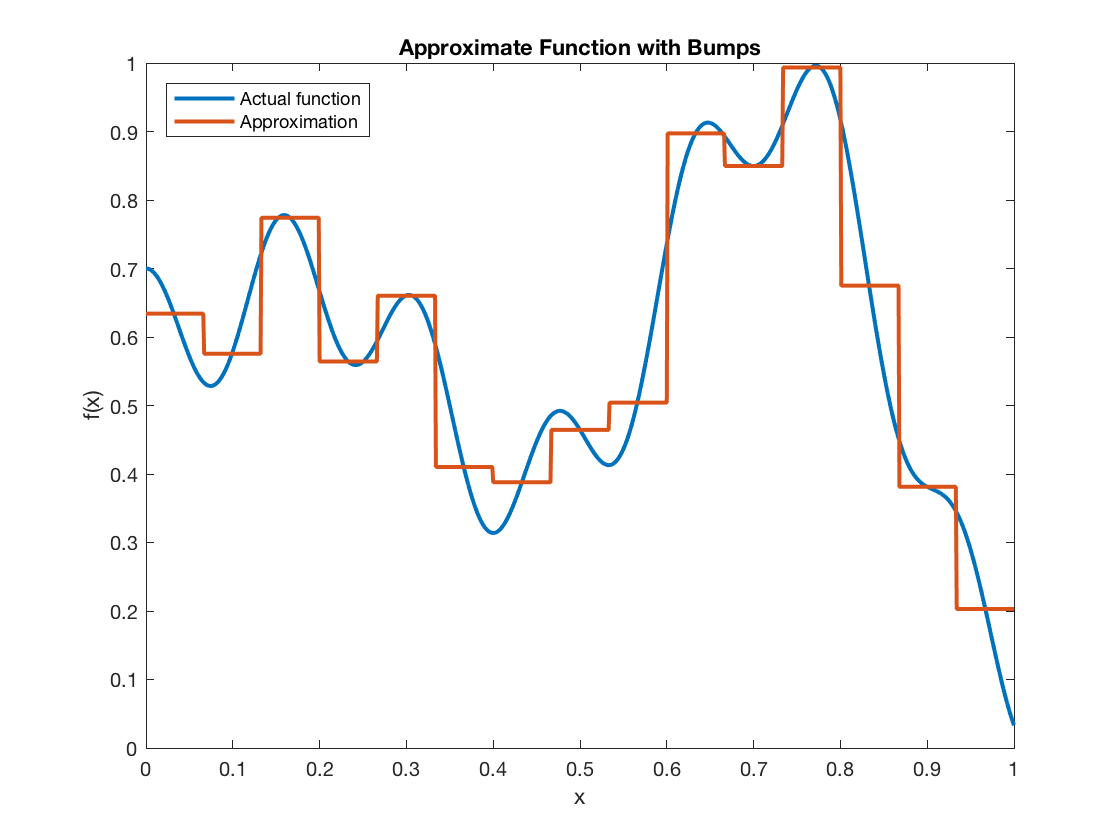
\includegraphics[width=.99\linewidth]{approximation.png}
  \caption{1D Function Approximation with Bumps}
  \label{fig:approximation_1d}
\end{subfigure}
\begin{subfigure}{.45\textwidth}
  \centering
  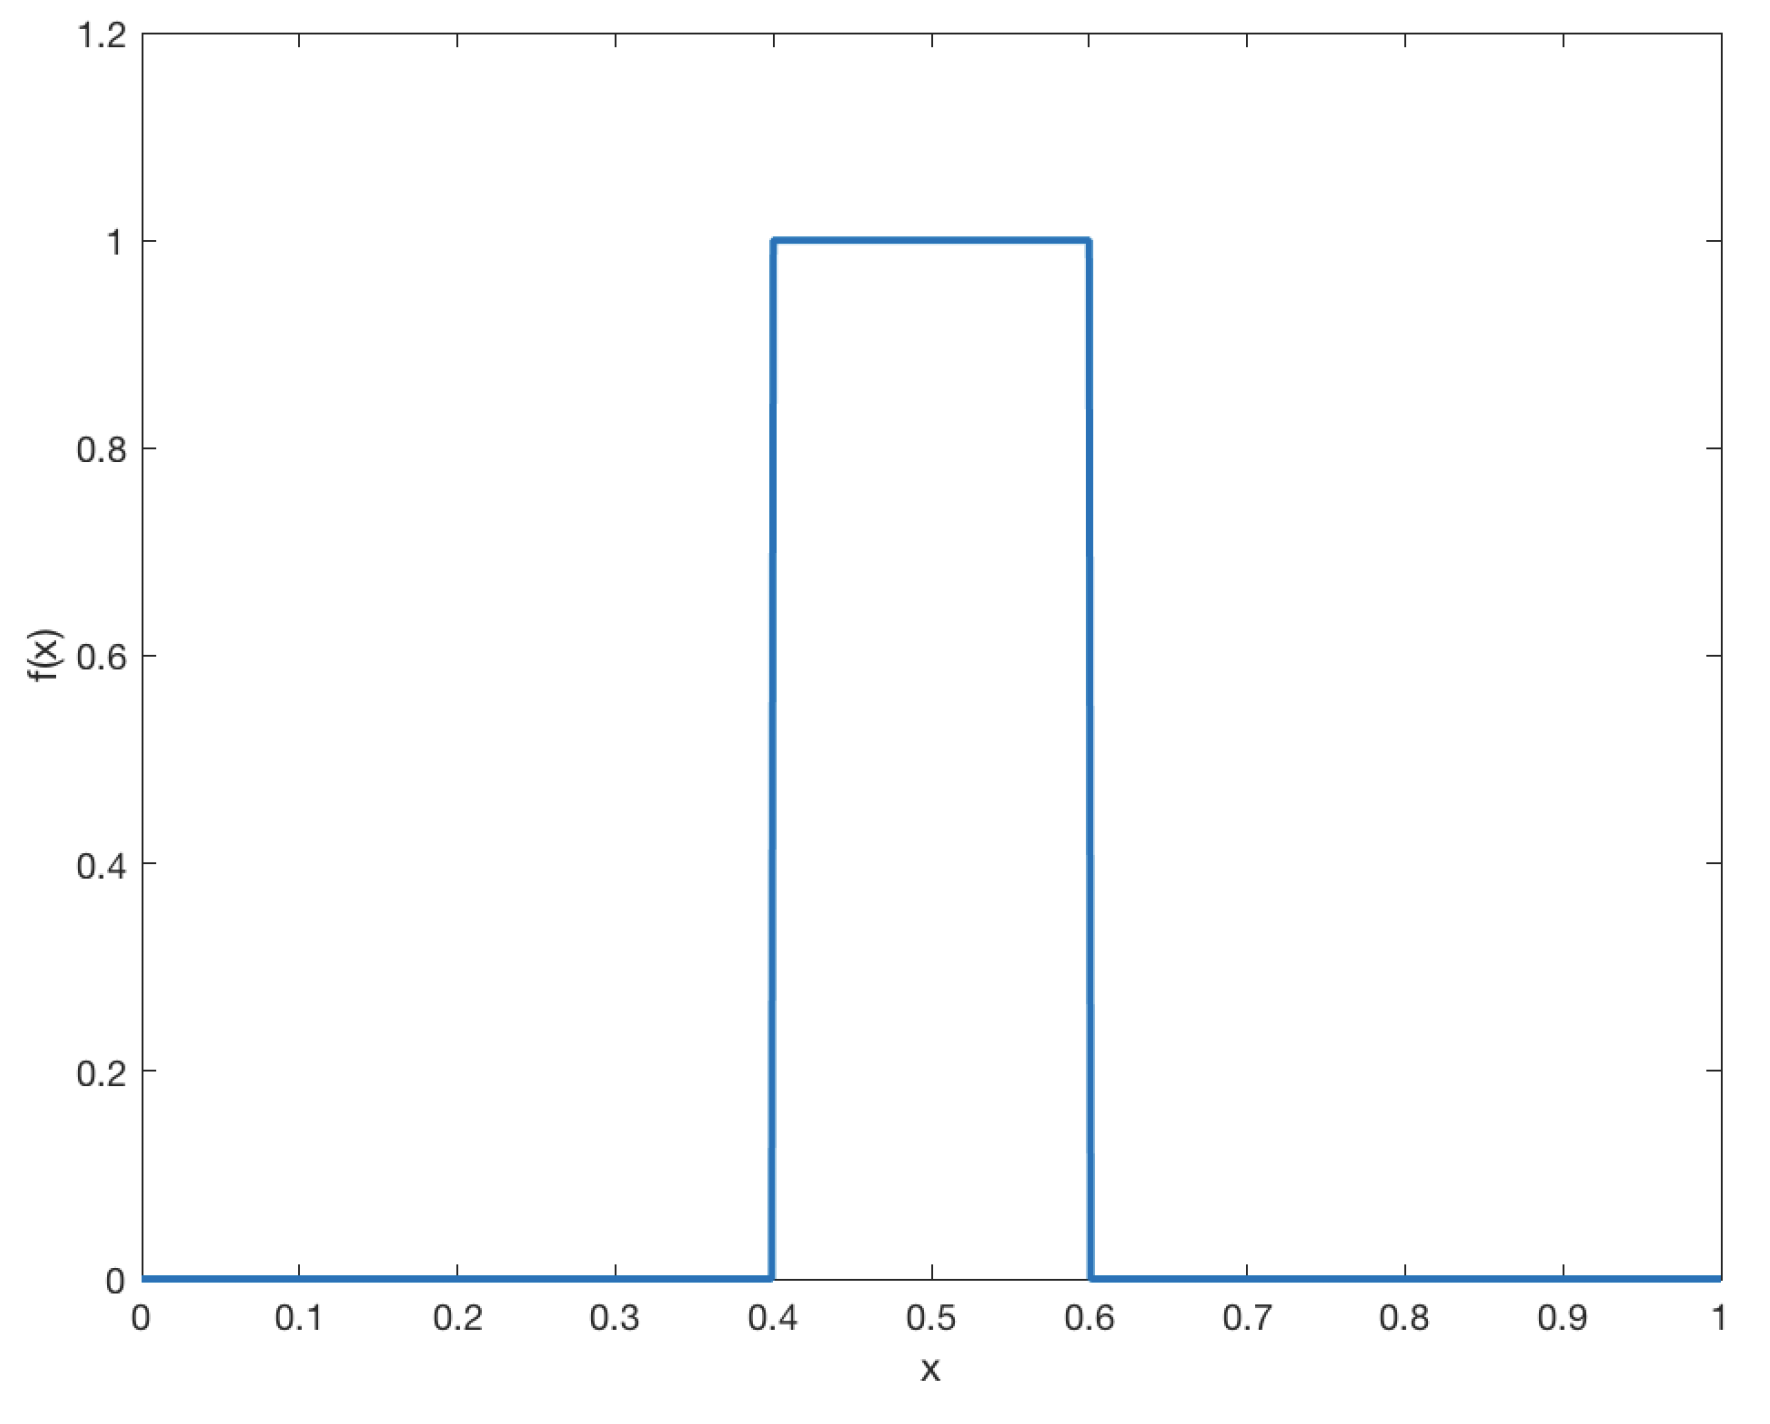
\includegraphics[width=.99\linewidth]{bump.png}
  \caption{1D Bump}
  \label{fig:bump}
\end{subfigure}
\begin{subfigure}{.45\textwidth}
  \centering
  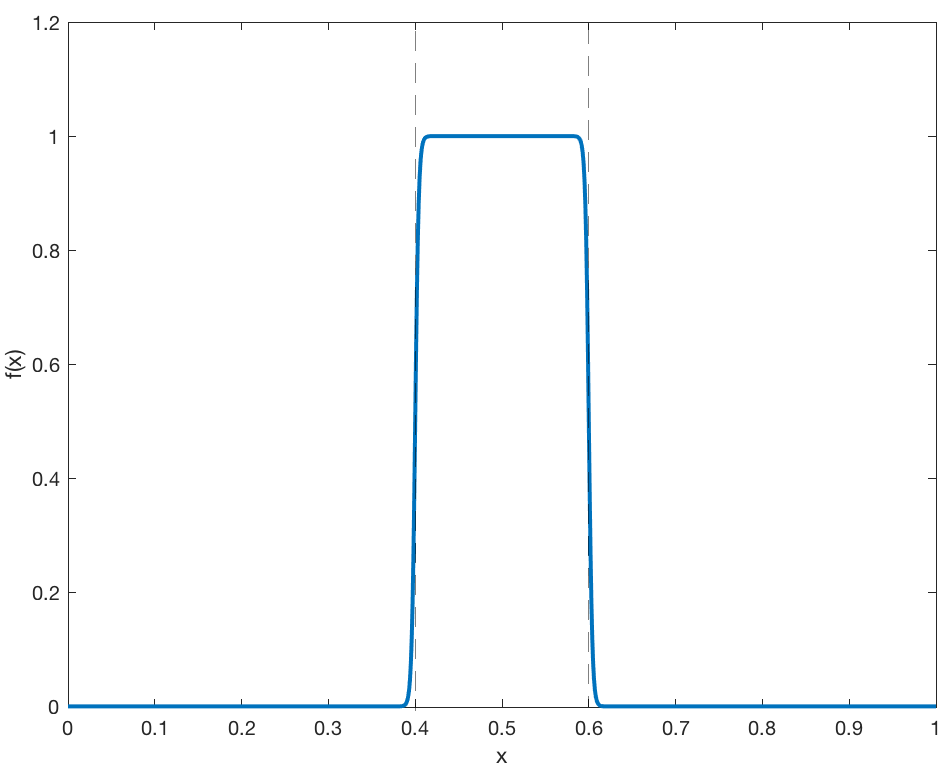
\includegraphics[width=.99\linewidth]{bump1.png}
  \caption{Approximation example}
  \label{fig:bump1}
\end{subfigure}%
\caption{Illustration of Function Approximation with Bumps}
\label{fig:bump_appro}
\end{figure}

\textbf{a.} Assuming sigmoid activation function is used, design a single layer NN with one input and one output to approximate the bump function shown in Fig.~\ref{fig:bump}. An example of a reasonable approximation using a single layer NN is show in in Fig.~\ref{fig:bump1}. Try to replicate it as closely as possible. (Hint: consider the bump as a combination of a step-up function and a step-down function). Implement it in the language of your choice and plot your approximation. Draw your NN architecture with all weights and bias values. Empirically, what is the minimum number of hidden neurons you need to make such approximation? 

\textbf{b.} Specify what parameters in your NN determine (1) the steepness of the step-up and step-down part of the bump, (2) the step-up and step-down locations (x-coordinates), (3) the height of the bump.

\begin{figure}[h!]
\centering
\begin{subfigure}{.49\textwidth}
  \centering
  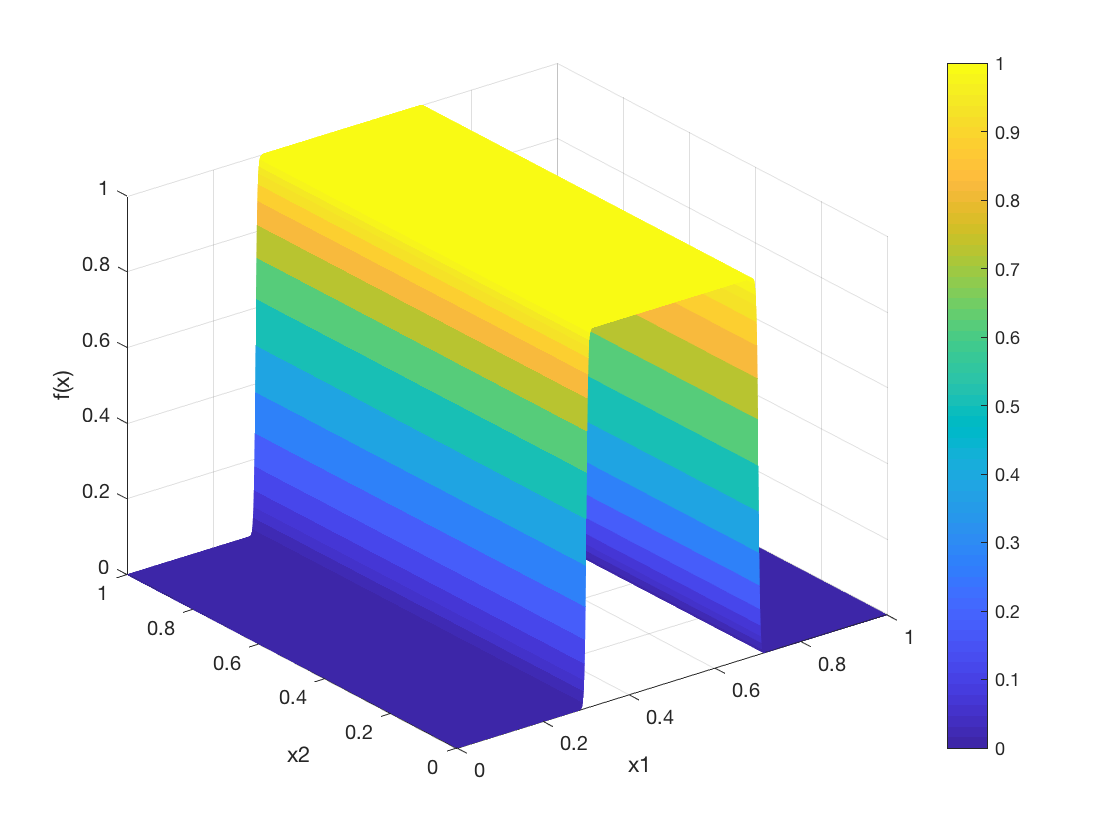
\includegraphics[width=.99\linewidth]{2d_bump.png}
  \caption{An approximation of a bump function}
  \label{fig:2d_bump}
\end{subfigure}
\begin{subfigure}{.49\textwidth}
  \centering
  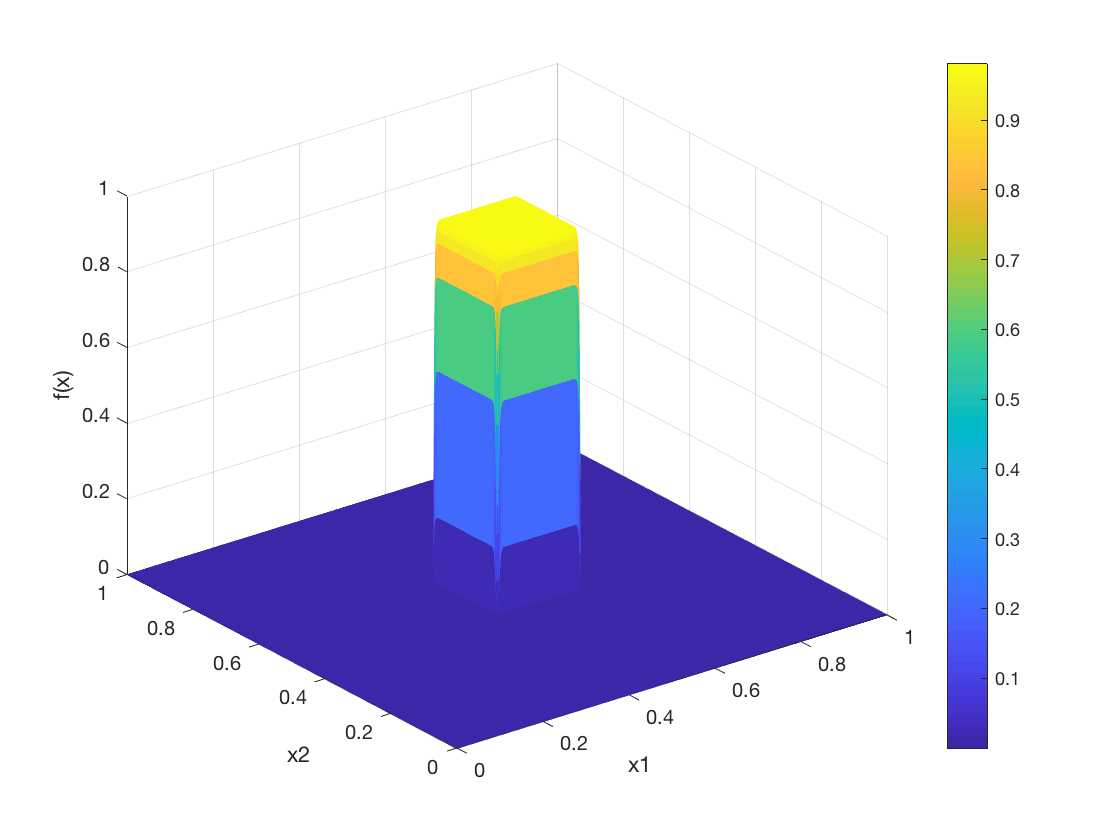
\includegraphics[width=.99\linewidth]{2d_peak.png}
  \caption{An approximation of a tower function}
  \label{fig:2d_peak}
\end{subfigure}%
\caption{Function Approximation with Two Inputs and One Output}
\label{fig:bump_appro}
\end{figure}

\subsection{}
Now we consider any function with two inputs and one output. We want to show that we can approximate it with a two-layer NN. 

\textbf{a.} Design a single layer NN with two inputs $x_1, x_2$, and one output $f(\textbf{x})$ to approximate a bump function in 2D. The bump goes up at $x_1 = 0.3$ and goes down at $x_1 = 0.7$. The height of the bump is $1$. An example of a reasonable approximation using a single layer NN is shown in Fig.~\ref{fig:2d_bump}. Try to replicate it as closely as possible. Implement it in the language of your choice and plot your approximation. Draw your NN architecture with all weights and bias values. Do not include any edge with zero weight. Empirically, what is the minimum number of hidden neurons you need to make such approximation? 

\textbf{b.} Design a two-layer NN with two inputs $x_1, x_2$, and one output $f(\textbf{x})$ to approximate a 2D tower function. The base of the tower is a square centered at $(0.5, 0.5)$ with side length $0.2$. The height of the tower is $1$. An example of a reasonable approximation using a two-layer NN is shown in Fig.~\ref{fig:2d_peak}. Try to replicate it as closely as possible. Implement it in the language of your choice and plot your approximation. (Hint: consider adding a $x_1$ direction bump and a $x_2$ direction bump together; you only need one hidden neuron in the second hidden layer--carefully tune the weights and bias of the second layer). Draw your NN architecture with all weights and bias values. Do not include any edge with zero weight. Empirically, what is the minimum number of 1st-layer hidden neurons you need to make such approximation? 

\textbf{c.} Suppose you have a 2D function $f(x_1, x_2)$ defined on a unit square ($x_1, x_2 \in \left [0,1 \right ]$). The maximum absolute value of the gradient for both directions is $t$. You want to approximate this function with a collection of tower functions similar to the one in part \textbf{b}. More specifically, we divide the unit square into a $n\times n$ grid. The towers are step functions that are centered at grid points, and each has width and depth $1/n$. You are allowed to adjust the height of each tower (this is identical incidentally to adjusting the pixels of a coarser image to represent a finer image). So we will have in total $n^2$ tower functions. And you want to make sure that the maximum error for each tower function used is $\epsilon$. What is the minimum number of tower functions that can guarantee to make such approximation for all possible function $f$ that satisfies the conditions? (Hint: think about the worst case for $f$.) Using the result from part \textbf{b}, what can you say about the relationship between the gradient limit, error bound, and the total required hidden neuron number?

\section{EM}
Suppose there are two tiny laundry machines in your Duke dorm and one of them is broken $\theta_1$ proportion of the time and the other is broken $\theta_2$ proportion of the time. Every time when a machine is broken, it simply takes your money and does not start. Each time you put money in the machine, the probability it will run is independent of what happened any other time you ran the machine. You never get a choice which machine you put yours in because the other one is always full when you go there. You went to the laundry room $m$ times this year, and in each visit, you got to use one of laundry machine at random. You always have way too many clothes, so you had to use whatever machine you got that day for $n$ times to wash all your clothes. (You only brought money for $n$ laundry cycles so you just have to wear the dirty clothes if the machine is broken for various cycles, hopefully no one will notice how smelly you are.) You recorded the number of successful cycles and the number of failed cycles (that sum to $n$). At the end of the year, your RA finally decided to report the problem and she asked you for the probability of failure for both machines. If you had recorded which machine you used every time, you would have had complete information and been able to estimate $\theta_1$ and $\theta_2$ in closed form. Sadly you were too lazy to do that, thus having to estimate these probabilities in a harder way. Luckily you learned a possible approach to address this problem from your favorite machine learning class---you can assign weights $w_i$ to each \textbf{laundry visit}, according to how likely it is done on machine 1 or machine 2.

\textbf{a.} Use EM algorithm to derive the estimation.

\textbf{b.} Implement the EM algorithm to estimate $\theta$ in the language of your choice. In your data simulation, set $m = 6, n = 100, \theta_1 = 0.8, \theta_2 = 0.3$. Show the progress of your estimation. 


\section{Clustering}

\begin{figure}[h!]
\centering
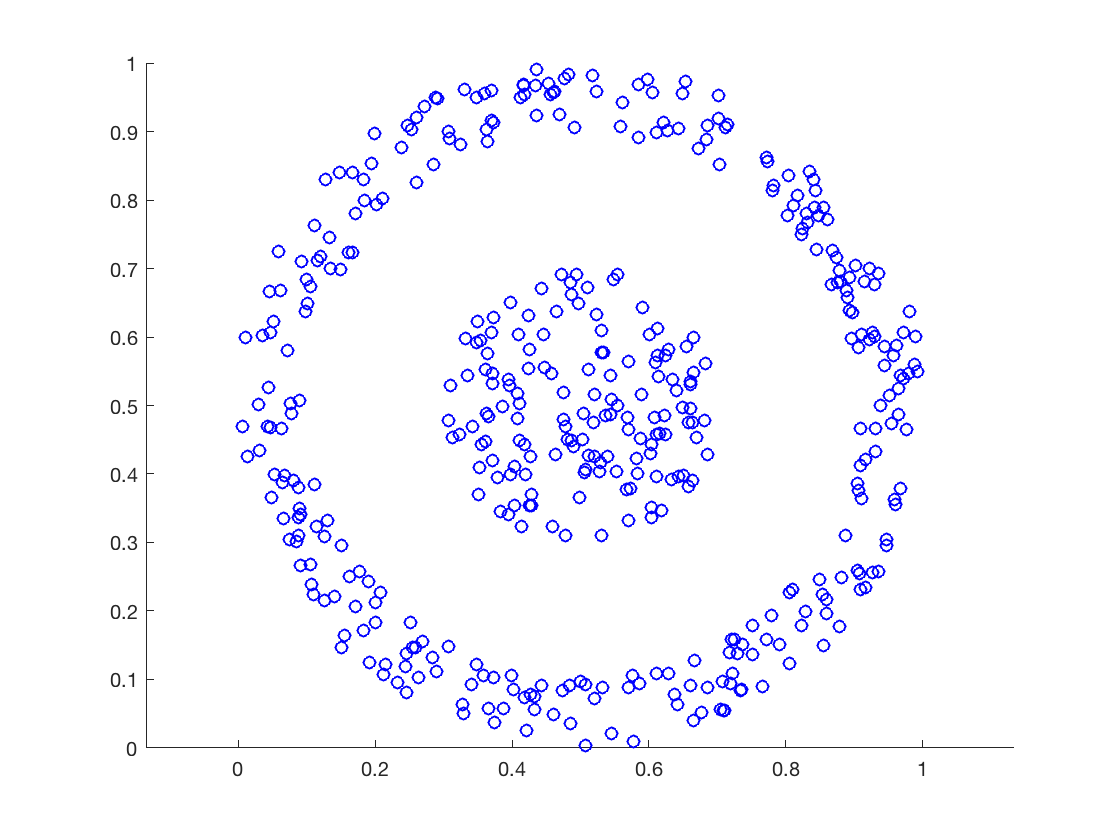
\includegraphics[scale=0.25]{cluster_data.png}
\caption{Dataset for Clustering}
\label{fig:cluster}
\end{figure}

\textbf{a.} Implement the k-means algorithm in the language of your choice. The arguments of your function are $k$ and the input dataset. Return both the group assignment for each point in the dataset, as well as the mean $\mu_j$ for each group. You can initialize each mean by randomly selecting a point from the input data.

\textbf{b.} Implement hierarchical agglomerative clustering algorithm in the language of your choice. The arguments of your function are $k$ and the input dataset. Return the group assignment for each point in the dataset

\textbf{c.} Run your algorithms developed in part \textbf{a} and part \textbf{b} on the dataset shown in Fig.~\ref{fig:cluster}, with $k = 2$. Which one performs better? Explain possible reasons for this discrepancy.

\textbf{d.} How can you pre-process the dataset to help boost the performance of the weaker algorithm in part \textbf{c}?

\end{document}
